\begin{tcolorbox}[
    colback=SkyBlue!5,
    colframe=blue!20,
    boxrule=1pt,
    arc=2pt,
    width=\textwidth,
    breakable
]
  \begin{minipage}[t]{0.48\textwidth}
    \centering
    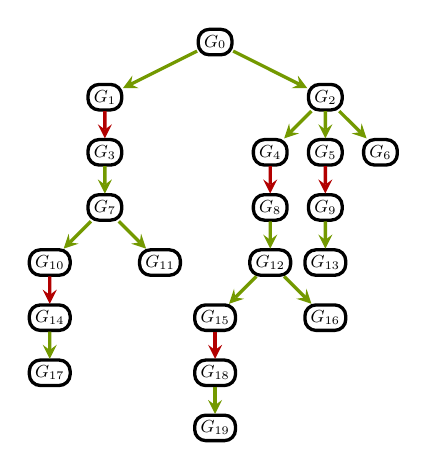
\begin{tikzpicture}[
    scale=0.7,
    transform shape,
    >=stealth,
    node distance=2.2cm and 2.5cm,
    hypernode/.style={draw, rectangle, rounded corners=4pt, very thick, inner sep=3pt, font=\small\bfseries},
    event/.style={draw=none, font=\normalsize},
    rf/.style={->, thick, dashed, green!60!black},
    co/.style={->, thick, dotted, red!80!black},
    graph box/.style={draw, rectangle, rounded corners=4pt, thick, minimum width=1.4cm, minimum height=1cm, inner sep=0.1cm, minimum size=0cm},
    edge label/.style={midway, very thick, fill=white, font=\footnotesize, inner sep=1pt},
    graph box yellow/.style={graph box, dashed},
    graph box blue/.style={graph box},
    every node/.style={transform shape},
    edge-t1/.style={->, very thick, lime!60!black},
    edge-t2/.style={->, very thick, red!70!black},
    circ-label-t1/.style={text=black, inner sep=1pt, font=\normalsize, scale=1.2},
    circ-label-t2/.style={text=black, inner sep=1pt, font=\normalsize, scale=1.2}
]


\node[hypernode] (G0) at (0,0) {$G_0$};

\node[hypernode] (G1) at (-2,-1) {$G_1$};

\node[hypernode] (G2) at (2,-1) {$G_2$};

\node[hypernode] (G3) at (-2,-2) {$G_3$};

\node[hypernode] (G4) at (1,-2) {$G_4$};

\node[hypernode] (G5) at (2,-2) {$G_5$};

\node[hypernode] (G6) at (3,-2) {$G_6$};

\node[hypernode] (G7) at (-2,-3) {$G_7$};

\node[hypernode] (G8) at (1,-3) {$G_8$};

\node[hypernode] (G9) at (2,-3) {$G_9$};

\node[hypernode] (G10) at (-3,-4) {$G_{10}$};

\node[hypernode] (G11) at (-1,-4) {$G_{11}$};

\node[hypernode] (G12) at (1,-4) {$G_{12}$};

\node[hypernode] (G13) at (2,-4) {$G_{13}$};

\node[hypernode] (G14) at (-3,-5) {$G_{14}$};

\node[hypernode] (G15) at (0,-5) {$G_{15}$};

\node[hypernode] (G16) at (2,-5) {$G_{16}$};

\node[hypernode] (G17) at (-3,-6) {$G_{17}$};

\node[hypernode] (G18) at (0,-6) {$G_{18}$};

\node[hypernode] (G19) at (0,-7) {$G_{19}$};


%% Hyper Edges

\draw[edge-t1] (G0) -- (G1);

\draw[edge-t1] (G0) -- (G2);

\draw[edge-t2] (G1) -- (G3);

\draw[edge-t1] (G2) -- (G4);

\draw[edge-t1] (G2) -- (G5);

\draw[edge-t1] (G2) -- (G6);

\draw[edge-t1] (G3) -- (G7);

\draw[edge-t2] (G4) -- (G8);

\draw[edge-t2] (G5) -- (G9);

\draw[edge-t1] (G7) -- (G10);

\draw[edge-t1] (G7) -- (G11);

\draw[edge-t1] (G8) -- (G12);

\draw[edge-t1] (G9) -- (G13);

\draw[edge-t2] (G10) -- (G14);

\draw[edge-t1] (G12) -- (G15);

\draw[edge-t1] (G12) -- (G16);

\draw[edge-t1] (G14) -- (G17);

\draw[edge-t2] (G15) -- (G18);

\draw[edge-t1] (G18) -- (G19);

\end{tikzpicture}
\captionof{figure}{The transition system $\mathcal{D}(\ref{ex:lll})$}
\label{lll-full}
  \end{minipage}
  \hfill
  \begin{minipage}[t]{0.48\textwidth}
    \centering
    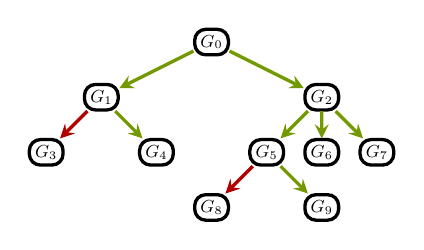
\begin{tikzpicture}[
    scale=0.7,
    transform shape,
    >=stealth,
    node distance=2.2cm and 2.5cm,
    hypernode/.style={draw, rectangle, rounded corners=4pt, very thick, inner sep=3pt, font=\small\bfseries},
    event/.style={draw=none, font=\normalsize},
    rf/.style={->, thick, dashed, green!60!black},
    co/.style={->, thick, dotted, red!80!black},
    graph box/.style={draw, rectangle, rounded corners=4pt, thick, minimum width=1.4cm, minimum height=1cm, inner sep=0.1cm, minimum size=0cm},
    edge label/.style={midway, very thick, fill=white, font=\footnotesize, inner sep=1pt},
    graph box yellow/.style={graph box, dashed},
    graph box blue/.style={graph box},
    every node/.style={transform shape},
    edge-t1/.style={->, very thick, lime!60!black},
    edge-t2/.style={->, very thick, red!70!black},
    circ-label-t1/.style={text=black, inner sep=1pt, font=\normalsize, scale=1.2},
    circ-label-t2/.style={text=black, inner sep=1pt, font=\normalsize, scale=1.2}
]


\node[hypernode] (G0) at (0,0) {$G_0$};

\node[hypernode] (G1) at (-2,-1) {$G_1$};

\node[hypernode] (G2) at (2,-1) {$G_2$};

\node[hypernode] (G3) at (-3,-2) {$G_3$};

\node[hypernode] (G4) at (-1,-2) {$G_4$};

\node[hypernode] (G5) at (1,-2) {$G_5$};

\node[hypernode] (G6) at (2,-2) {$G_6$};

\node[hypernode] (G7) at (3,-2) {$G_7$};

\node[hypernode] (G8) at (0,-3) {$G_8$};

\node[hypernode] (G9) at (2,-3) {$G_9$};



%% Hyper Edges

\draw[edge-t1] (G0) -- (G1);

\draw[edge-t1] (G0) -- (G2);

\draw[edge-t2] (G1) -- (G3);

\draw[edge-t1] (G1) -- (G4);

\draw[edge-t1] (G2) -- (G5);

\draw[edge-t1] (G2) -- (G6);

\draw[edge-t1] (G2) -- (G7);

\draw[edge-t2] (G5) -- (G8);

\draw[edge-t1] (G5) -- (G9);

\end{tikzpicture}
\captionof{figure}{The compressed transition system $\mathcal{D}(\ref{ex:lll})$}
\label{lll-comp}
  \end{minipage}
\begin{example}
Consider the following program.

\begin{equation*}
  \tag{\textsc{L+L+L}}
  \label{ex:lll}
  \inarr{ 
\lockInst{l} \\
\unlockInst{l} \\
}{ 
\lockInst{l} \\
\unlockInst{l} \\
}{
\lockInst{l} \\
\unlockInst{l} \\
}
\end{equation*}

This program consists of three threads, each of which attempts to acquire a lock and subsequently release it. It has $3!$ execution graphs. The complete $\mathcal{D}(\ref{ex:lll})$ tree of this program without tree compression is depicted in \cref{lll-full} and
with compression in \cref{lll-comp}.
With $B=5$, the uncompressed tree requires 20 clones and re-execution but the compressed tree only 10.
%When running \testor with $\mathcal{B} = 4$ over this tree, approximately 20 graph clonings and re-executions must take place per iteration. However, when running \testor with $\mathcal{B} = 5$ over the compressed $\mathcal{D}(\ref{ex:lll})$ tree, as depicted in \cref{lll-comp}, only approximately 10 graph clonings and re-executions are required, reflecting a twofold reduction in overhead.
\qed
\end{example}
\end{tcolorbox}
